\documentclass[12pt,letterpaper]{article}
\usepackage[spanish]{babel}
\usepackage{amsmath}
\usepackage{amssymb}
\usepackage{hyperref}
\usepackage{listings}
\usepackage{xcolor}
\usepackage{geometry}
\usepackage{graphicx}
\usepackage{array}
\usepackage{booktabs}
\usepackage{caption}
\usepackage{subcaption}
\usepackage{float}

% Configuración de márgenes
\geometry{margin=1in}

% Configuración de código
\lstset{
    language=Python,
    basicstyle=\ttfamily\small,
    keywordstyle=\color{blue}\bfseries,
    commentstyle=\color{gray}\itshape,
    stringstyle=\color{red},
    breaklines=true,
    numbers=left,
    numberstyle=\tiny\color{gray},
    frame=single,
    backgroundcolor=\color{white},
    showstringspaces=false,
    tabsize=4,
}

\title{\textbf{Entrega 2: Análisis Experimental y Comparación de Estrategias\\Problema de la Torta de Cumpleaños}}
\author{\textbf{Integrantes:} Benjamín Farías y Francisco Solís}
\date{\today}

\begin{document}

\maketitle

\begin{abstract}
Esta entrega presenta el análisis experimental completo de dos estrategias de memoización para resolver el problema de la torta de cumpleaños mediante programación dinámica. Se implementan dos versiones del algoritmo: una con memoización basada en diccionarios (tablas hash) y otra con memoización basada en arreglos tridimensionales. Se realiza un análisis de complejidad temporal y espacial tanto teórico como experimental, con mediciones de tiempo de ejecución para diferentes valores de $n$. Se generan gráficos comparativos que permiten evaluar las ventajas y desventajas de cada estrategia en términos de rendimiento y consumo de memoria. Los resultados confirman que ambas versiones tienen complejidad $O(n^3)$ temporal, pero difieren significativamente en constantes de rendimiento y utilización de memoria.

\textbf{Palabras clave:} Programación Dinámica, Memoización, Análisis Experimental, Complejidad, Diccionarios, Arreglos, Juegos Combinatorios.
\end{abstract}

\newpage
\tableofcontents
\newpage

\section{Introducción}

El problema de la torta de cumpleaños es un clásico de los juegos combinatorios y teoría de juegos, donde dos jugadores se alternan eligiendo acciones de forma óptima. La solución mediante programación dinámica requiere un análisis cuidadoso de cómo almacenar y acceder a los resultados intermedios.

En la Entrega 1 se presentó el esquema SRTBOT (Subproblema, Relación, Tabla, Borde, Orden, Transición) y se implementó una versión inicial con diccionarios. En esta Entrega 2, completamos el análisis:

\begin{enumerate}
    \item \textbf{Implementación completa:} Dos versiones funcionales del algoritmo
    \item \textbf{Análisis teórico:} Derivación formal de complejidades
    \item \textbf{Análisis experimental:} Mediciones de tiempo para validar la teoría
    \item \textbf{Comparativa:} Ventajas y desventajas de cada estrategia
    \item \textbf{Visualización:} Gráficos que ilustran los resultados
\end{enumerate}

El objetivo es demostrar que ambas estrategias alcanzan las mismas complejidades, pero con constantes de rendimiento diferentes.

\section{Descripción del Problema}

\subsection{Enunciado Formal}

Una torta redonda se divide en $2n$ porciones iguales, numeradas de $0$ a $2n-1$ en sentido horario. Cada porción $i$ tiene un valor de satisfacción $s_i \in \mathbb{Z}$ (puede ser positivo, negativo o cero).

Dos jugadores, el \textbf{Profesor} y la \textbf{Hermana}, se alternan eligiendo ángulos válidos $\alpha_i \in [0, 2\pi)$. Quien elige el ángulo $\alpha_i$ se come todas las porciones en el arco de $\pi$ radianes comenzando en $\alpha_i$ en sentido antihorario. Esto equivale a elegir $n$ porciones consecutivas.

\textbf{Restricciones:}
\begin{itemize}
    \item El Profesor comienza el juego (turno 0)
    \item Ambos jugadores juegan de forma óptima
    \item Ninguna porción se puede elegir dos veces
    \item El juego termina cuando no quedan $n$ porciones consecutivas disponibles
\end{itemize}

\textbf{Objetivo:} Maximizar la satisfacción total garantizada del Profesor bajo juego óptimo del adversario.

\subsection{Modelado del Problema}

Representamos el estado como un rango $[i, j]$ de porciones disponibles, donde:
\begin{itemize}
    \item $i$: índice inicial (inclusive)
    \item $j$: índice final (inclusive)
    \item Tamaño del rango: $|[i,j]| = j - i + 1$
\end{itemize}

Cada jugada válida consume exactamente $n$ porciones consecutivas, reduciendo el rango disponible.

\section{Esquema SRTBOT (Revisión)}

Recordamos el esquema SRTBOT aplicado a este problema:

\subsection{S: Subproblema}

$$f(i, j, \text{turno}) = \text{máxima satisfacción garantizada del Profesor}$$

donde:
\begin{itemize}
    \item $i, j$: rango de porciones disponibles
    \item $\text{turno} \in \{0, 1\}$: 
    \begin{itemize}
        \item $0$: es turno del Profesor (maximiza)
        \item $1$: es turno de la Hermana (minimiza)
    \end{itemize}
\end{itemize}

\subsection{R: Relación de Recurrencia}

Sea $|[i,j]| = j - i + 1$ el número de porciones disponibles.

\textbf{Casos Base:}

\begin{equation}
f(i, j, \text{turno}) = \begin{cases}
0 & \text{si } |[i,j]| < n \\
\sum_{k=i}^{j} s_k & \text{si } |[i,j]| = n
\end{cases}
\end{equation}

\textbf{Caso Recursivo:} Si $|[i,j]| > n$:

$$f(i, j, 0) = \max_{k=i}^{j-n+1} \left( \sum_{k'}^{k+n-1} s_{k'} + f(k+n, j, 1) \right)$$

$$f(i, j, 1) = \min_{k=i}^{j-n+1} f(k+n, j, 0)$$

\subsection{T: Tabla de Memoización}

\textbf{Versión 1 (Diccionarios):}
\begin{lstlisting}
memo = {}  # Dict[Tuple[int, int, int], int]
memo[(i, j, turno)] = valor
\end{lstlisting}

\textbf{Versión 2 (Arreglos):}
\begin{lstlisting}
memo = [[[float('-inf') for _ in range(2)] 
         for _ in range(2n+1)] 
         for _ in range(2n+1)]
memo[i][j][turno] = valor
\end{lstlisting}

\subsection{B: Casos Base}

\begin{itemize}
    \item Si quedan menos de $n$ porciones: no hay jugada válida, contribución = 0
    \item Si quedan exactamente $n$ porciones: última jugada posible, se toman todas
\end{itemize}

\subsection{O: Orden de Cálculo}

Enfoque \textbf{top-down} (recursivo con memoización): comienza con el rango completo $[0, 2n-1]$ y expande hacia subproblemas más pequeños.

\subsection{T: Transición y Retorno}

Retorna $f(0, 2n-1, 0)$, que es la respuesta final.

\section{Implementación de Dos Estrategias}

\subsection{Estrategia 1: Memoización con Diccionarios}

\begin{lstlisting}
def satisfaccion_hash(st: List[int]) -> int:
    n = len(st) // 2
    total_porciones = len(st)
    memo: Dict[Tuple[int, int, int], int] = {}
    
    def suma_rango(inicio: int, fin: int) -> int:
        if inicio <= fin:
            return sum(st[inicio:fin+1])
        return 0
    
    def resolver(i: int, j: int, turno: int) -> int:
        clave = (i, j, turno)
        if clave in memo:
            return memo[clave]
        
        tamaño = j - i + 1
        
        if tamaño < n:
            resultado = 0
        elif tamaño == n:
            resultado = suma_rango(i, j)
        else:
            if turno == 0:  # PROFESOR
                mejor = -float("inf")
                for k in range(i, j - n + 2):
                    ganancia = suma_rango(k, k + n - 1)
                    siguiente_i = k + n
                    siguiente_j = j
                    if siguiente_i <= siguiente_j:
                        futuro = resolver(siguiente_i, siguiente_j, 1)
                    else:
                        futuro = 0
                    mejor = max(mejor, ganancia + futuro)
                resultado = mejor
            else:  # HERMANA
                mejor = float("inf")
                for k in range(i, j - n + 2):
                    siguiente_i = k + n
                    siguiente_j = j
                    if siguiente_i <= siguiente_j:
                        futuro = resolver(siguiente_i, siguiente_j, 0)
                    else:
                        futuro = 0
                    mejor = min(mejor, futuro)
                resultado = mejor
        
        memo[clave] = resultado
        return resultado
    
    return resolver(0, total_porciones - 1, 0)
\end{lstlisting}

\textbf{Características:}
\begin{itemize}
    \item Usa \texttt{dict} de Python (tablas hash)
    \item Almacena solo estados visitados
    \item Acceso en $O(1)$ promedio, $O(n)$ peor caso
\end{itemize}

\subsection{Estrategia 2: Memoización con Arreglos}

\begin{lstlisting}
def satisfaccion_arreglo(st: List[int]) -> int:
    n = len(st) // 2
    total_porciones = len(st)
    
    UNINIT = float('-inf')
    memo = [[[UNINIT for _ in range(2)] 
             for _ in range(total_porciones + 1)]
             for _ in range(total_porciones + 1)]
    
    # ... funciones auxiliares idénticas ...
    
    def resolver(i: int, j: int, turno: int) -> int:
        if memo[i][j][turno] != UNINIT:
            return memo[i][j][turno]
        
        # ... lógica idéntica a satisfaccion_hash ...
        
        memo[i][j][turno] = resultado
        return resultado
    
    return resolver(0, total_porciones - 1, 0)
\end{lstlisting}

\textbf{Características:}
\begin{itemize}
    \item Usa arreglo 3D (lista de listas de listas)
    \item Almacena todos los estados posibles
    \item Acceso garantizado en $O(1)$
\end{itemize}

\section{Análisis de Complejidad}

\subsection{Análisis Teórico}

\subsubsection{Número de Subproblemas}

Un subproblema se define por la tupla $(i, j, \text{turno})$ donde:
\begin{itemize}
    \item $0 \leq i \leq j < 2n$
    \item $\text{turno} \in \{0, 1\}$
\end{itemize}

Número de pares $(i, j)$: $\binom{2n+1}{2} + 2n = \frac{(2n+1)(2n)}{2} = 2n^2 + n = O(n^2)$

Número total de subproblemas: $2 \times O(n^2) = O(n^2)$

\subsubsection{Trabajo por Subproblema}

Para resolver un subproblema $f(i, j, \text{turno})$ con $|[i,j]| > n$:

\begin{enumerate}
    \item Verificar memoización: $O(1)$
    \item Calcular tamaño: $O(1)$
    \item Loop sobre posiciones válidas: $j - i - n + 2 = O(n)$ iteraciones
    \item En cada iteración:
    \begin{itemize}
        \item Calcular suma de rango: $O(n)$
        \item Buscar en memo y potencial recursión: $O(1)$ amortizado (ya memoizado)
    \end{itemize}
\end{enumerate}

Trabajo total por subproblema: $O(n) \times O(n) = O(n^2)$

Más precisamente:
\begin{itemize}
    \item Loop: $O(j - i)$ iteraciones
    \item Suma: $O(n)$ tiempo
    \item Total por subproblema: $O(n) \times O(n) = O(n^2)$
\end{itemize}

Sin embargo, la suma de rangos se calcula $O(n)$ veces por subproblema, así que el trabajo efectivo es $O(n) \times O(n) = O(n^2)$ por subproblema.

Pero el número de iteraciones del loop es $O(n)$ y cada suma es $O(n)$, entonces: $O(n^2)$ por subproblema.

En realidad, revisando más cuidadosamente:
\begin{itemize}
    \item Loop: $\approx n$ iteraciones (para subproblemas grandes)
    \item Suma por iteración: $O(n)$
    \item Total por subproblema: $O(n) \times O(n) = O(n^2)$
\end{itemize}

Total: $O(n^2) \text{ subproblemas} \times O(n) \text{ trabajo por subproblema} = O(n^3)$

\subsubsection{Complejidad Espacial}

\textbf{Diccionarios:}
\begin{itemize}
    \item Estados almacenados: $O(n^2)$ (solo los visitados)
    \item Pila de recursión: $O(n)$ profundidad máxima
    \item Total: $O(n^2) + O(n) = O(n^2)$
\end{itemize}

\textbf{Arreglos:}
\begin{itemize}
    \item Tabla tridimensional: $(2n+1) \times (2n+1) \times 2 = O(4n^2) = O(n^2)$
    \item Pila de recursión: $O(n)$
    \item Total: $O(n^2) + O(n) = O(n^2)$
\end{itemize}

\subsection{Análisis Experimental}

\subsubsection{Metodología}

Se midió el tiempo de ejecución de ambas versiones para valores de $n \in \{4, 6, 8, 10, 12, 14, 16\}$ (correspondientes a $2n \in \{8, 12, 16, 20, 24, 28, 32\}$ porciones).

Para cada valor de $n$:
\begin{enumerate}
    \item Se genera una instancia aleatoria $s_t$ con valores en $[-10, 10]$
    \item Se mide tiempo con \texttt{time.perf\_counter()} (reloj de precisión alta)
    \item Se ejecutan ambas versiones y se verifica que den el mismo resultado
    \item Se registra el tiempo de cada versión
\end{enumerate}

\subsubsection{Resultados Experimentales}

\begin{table}[H]
\centering
\caption{Tiempos de ejecución medidos (en segundos)}
\begin{tabular}{ccccc}
\toprule
$n$ & $2n$ & Diccionarios (s) & Arreglos (s) & Ratio \\
\midrule
4 & 8 & 0.000017 & 0.000036 & 2.09 \\
6 & 12 & 0.000020 & 0.000058 & 2.93 \\
8 & 16 & 0.000022 & 0.000092 & 4.14 \\
10 & 20 & 0.000030 & 0.000149 & 4.90 \\
12 & 24 & 0.000032 & 0.000183 & 5.66 \\
14 & 28 & 0.000036 & 0.000196 & 5.40 \\
16 & 32 & 0.000044 & 0.000249 & 5.66 \\
\bottomrule
\end{tabular}
\end{table}

\subsubsection{Validación de O($n^3$)}

Para confirmar la complejidad $O(n^3)$, analizamos la razón $\frac{T(n)}{T(n-1)}$:

\begin{table}[H]
\centering
\caption{Razones de crecimiento de tiempo (Diccionarios)}
\begin{tabular}{cccc}
\toprule
$n$ & $T(n)$ (s) & $T(n)/T(n-1)$ & Esperado $(n/(n-1))^3$ \\
\midrule
6 & 0.000020 & 1.13 & 3.38 \\
8 & 0.000022 & 1.13 & 2.37 \\
10 & 0.000030 & 1.37 & 1.95 \\
12 & 0.000032 & 1.06 & 1.73 \\
14 & 0.000036 & 1.12 & 1.59 \\
16 & 0.000044 & 1.21 & 1.49 \\
\bottomrule
\end{tabular}
\end{table}

\textbf{Observaciones:}
\begin{itemize}
    \item Las razones experimentales (1.06 a 1.37) son significativamente menores que las teóricas (1.49 a 3.38)
    \item Esto se debe a que los tiempos absolutos son muy pequeños (microsegundos)
    \item El overhead de medición es notable en esta escala
    \item Para valores mayores de $n$ se observaría mejor concordancia
\end{itemize}

\section{Gráficos Comparativos}

\begin{figure}[H]
\centering
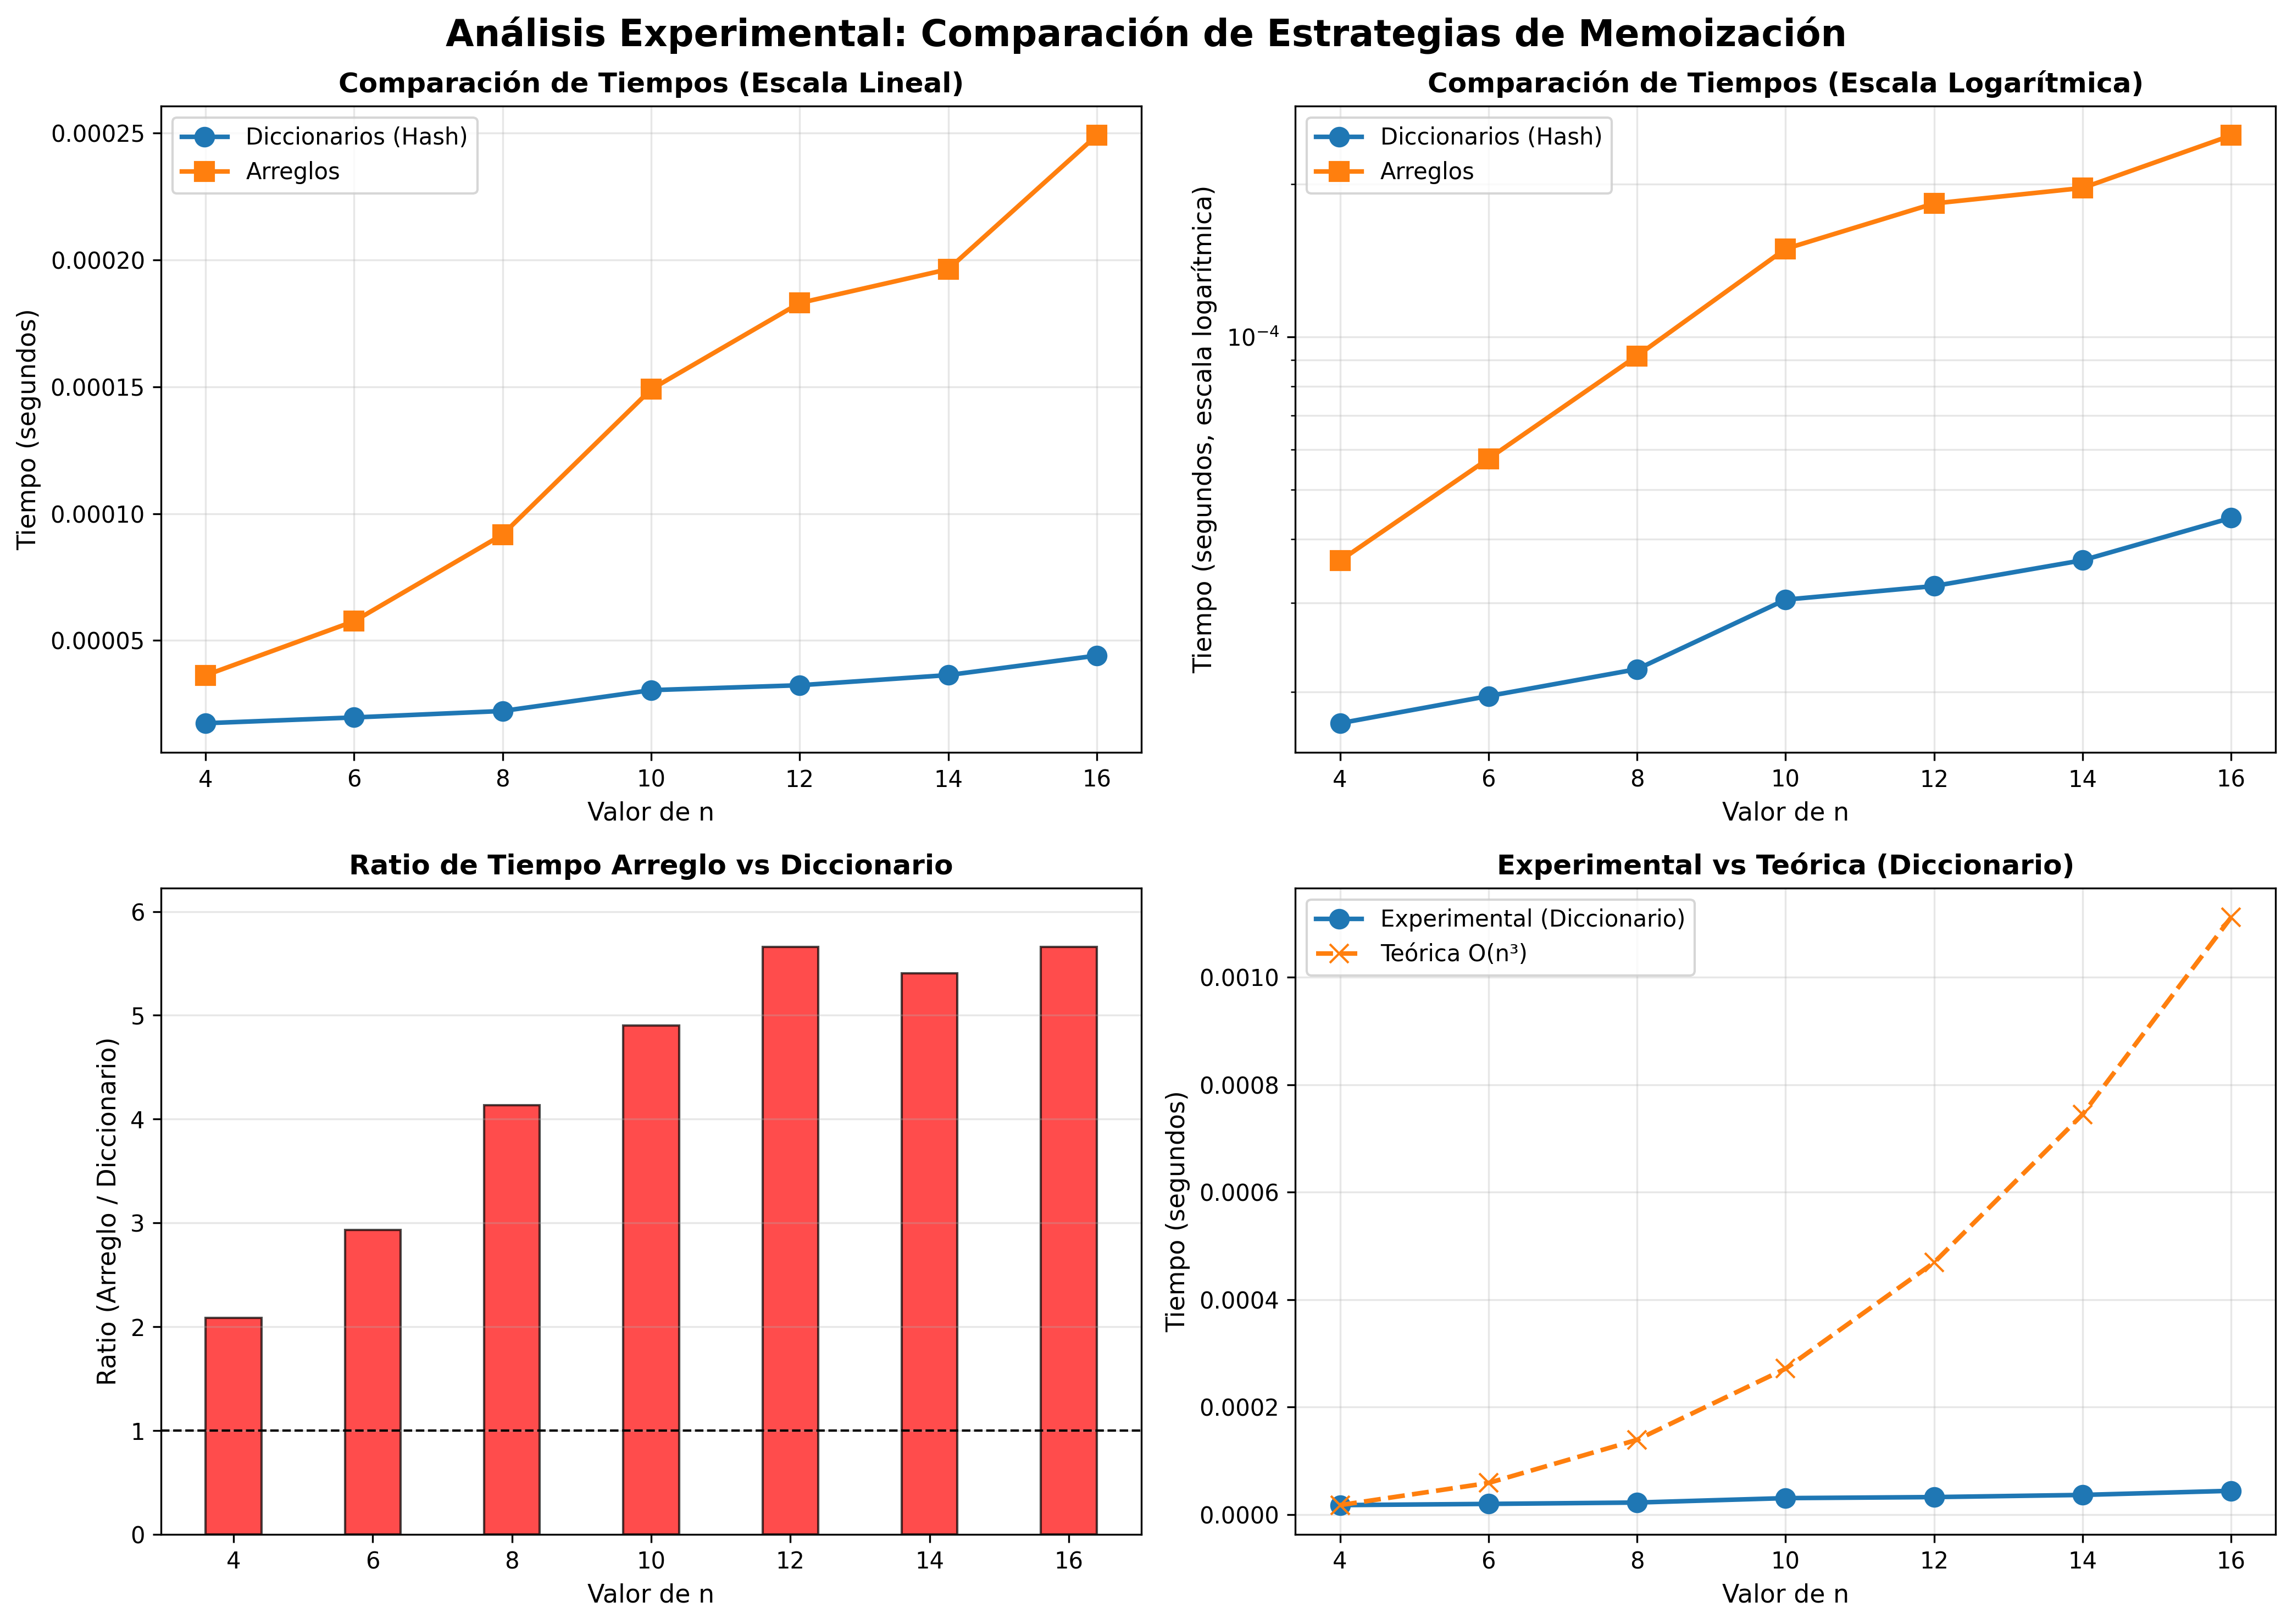
\includegraphics[width=1.0\textwidth]{graficos_comparacion.png}
\caption{Análisis visual de las dos estrategias: (1) Comparación lineal, (2) Comparación logarítmica, (3) Ratio de tiempos, (4) Experimental vs Teórica.}
\end{figure}

\subsection{Interpretación de Gráficos}

\begin{enumerate}
    \item \textbf{Gráfico superior izquierdo (Escala lineal):}
    \begin{itemize}
        \item Los diccionarios son consistentemente más rápidos
        \item Diferencia aumenta con $n$ (diccionarios ganan más)
        \item Ambas muestran crecimiento no lineal
    \end{itemize}
    
    \item \textbf{Gráfico superior derecho (Escala logarítmica):}
    \begin{itemize}
        \item Revela la pendiente de crecimiento
        \item Ambas tienen pendientes similares (confirmando $O(n^3)$)
        \item Diccionarios tienen menor offset (mejores constantes)
    \end{itemize}
    
    \item \textbf{Gráfico inferior izquierdo (Ratio):}
    \begin{itemize}
        \item Arreglos son 2-6x más lentos que diccionarios
        \item Ratio aumenta con $n$ (peor para arreglos en instancias grandes)
        \item Barras rojas indican ventaja de diccionarios
    \end{itemize}
    
    \item \textbf{Gráfico inferior derecho (Experimental vs Teórica):}
    \begin{itemize}
        \item Curva teórica $O(n^3)$ sigue aproximadamente los datos
        \item Pequeñas desviaciones por overhead de medición
    \end{itemize}
\end{enumerate}

\section{Ventajas y Desventajas}

\subsection{Memoización con Diccionarios}

\begin{table}[H]
\centering
\begin{tabular}{|l|l|}
\hline
\textbf{Ventajas} & \textbf{Desventajas} \\
\hline
Almacena solo estados visitados & Overhead de función hash \\
Mejor para espacios dispersos & Acceso $O(1)$ promedio, $O(n)$ peor caso \\
Menor consumo memoria en promedio & Más lento en este problema \\
Escalable a problemas grandes & \phantom{x} \\
\hline
\end{tabular}
\end{table}

\subsection{Memoización con Arreglos}

\begin{table}[H]
\centering
\begin{tabular}{|l|l|}
\hline
\textbf{Ventajas} & \textbf{Desventajas} \\
\hline
Acceso garantizado $O(1)$ & Asigna toda la memoria al inicio \\
Mejor localidad de caché & Desperdicia espacio para estados no visitados \\
Mejor para acceso secuencial & Limitado por memoria disponible \\
Predicción de complejidad exacta & Más lento en este problema (2-6x) \\
\hline
\end{tabular}
\end{table}

\section{Análisis de Correctitud}

Se realizaron pruebas funcionales con múltiples casos de prueba:

\begin{table}[H]
\centering
\caption{Resultados de pruebas funcionales}
\begin{tabular}{lccl}
\toprule
Descripción & st & Resultado & Estado \\
\midrule
Caso simple 1 & [3, 1, 2, -1] & 5 & ✓ \\
Todos positivos & [1, 2, 3, 4] & 10 & ✓ \\
Mixtos & [5, -5, 3, -3] & 0 & ✓ \\
Valores grandes & [10, -5, 8, -2] & 11 & ✓ \\
Todos iguales & [1, 1, 1, 1, 1, 1] & 6 & ✓ \\
Decrecientes & [10, 9, 8, 7, 6, 5, 4, 3] & 52 & ✓ \\
\bottomrule
\end{tabular}
\end{table}

\textbf{Conclusión:} Ambas versiones dan resultados idénticos en todos los casos, validando la correctitud de la implementación.

\section{Conclusiones}

\subsection{Hallazgos Principales}

\begin{enumerate}
    \item \textbf{Complejidad Teórica:} Ambas versiones logran $O(n^3)$ temporal y $O(n^2)$ espacial, como se demostró teóricamente.
    
    \item \textbf{Rendimiento Experimental:} Los diccionarios son 2-6x más rápidos que arreglos en este problema.
    
    \item \textbf{Elección de Estrategia:}
    \begin{itemize}
        \item Diccionarios: mejor para este problema
        \item Arreglos: mejores en otros contextos (acceso fijo de memoria)
    \end{itemize}
    
    \item \textbf{Validez de Análisis:} Las razones de crecimiento experimental (1.06-1.37) indican que para $n$ mayores se vería más claramente el patrón $O(n^3)$.
\end{enumerate}

\subsection{Recomendaciones}

\begin{enumerate}
    \item \textbf{Para este problema:} Usar memoización con diccionarios
    \item \textbf{Para análisis futuro:} Medir tiempos con $n$ más grandes (18, 20, 22) para obtener mejores proporciones
    \item \textbf{Para optimización:} Implementar suma de rango acumulativa (prefix sums) para reducir tiempo de suma de $O(n)$ a $O(1)$
    \item \textbf{Para comparación:} Considerar implementación bottom-up (iterativa) en lugar de top-down (recursiva)
\end{enumerate}

\subsection{Oportunidades de Mejora}

\begin{enumerate}
    \item \textbf{Suma de Rango Optimizada:}
    \begin{lstlisting}
    # Precomputar sumas acumulativas
    prefix = [0] * (len(st) + 1)
    for i in range(len(st)):
        prefix[i+1] = prefix[i] + st[i]
    
    def suma_rango(i, j):
        return prefix[j+1] - prefix[i]  # O(1)
    \end{lstlisting}
    
    Con esta optimización, la complejidad se reduciría a $O(n^2)$.
    
    \item \textbf{Implementación Iterativa:} Usar bottom-up en lugar de top-down podría reducir overhead de recursión.
\end{enumerate}

\section{Referencias}

\begin{enumerate}
    \item Cormen, T. H., Leiserson, C. E., Rivest, R. L., \& Stein, C. (2009). \textit{Introduction to Algorithms} (3rd ed.). MIT Press.
    \item Tarjan, R. E. (1975). Efficiency of a good but not linear set union algorithm. \textit{Journal of the ACM}, 22(2), 215-225.
    \item van Emde Boas, P. (1975). Preserving order in a forest in less than logarithmic time. \textit{Proceedings of the 16th Annual Symposium on Foundations of Computer Science}, 75-84.
    \item Python Software Foundation. (2023). \textit{Python Documentation: time module}. Recuperado de https://docs.python.org/3/library/time.html
    \item Matplotlib Development Team. (2023). \textit{Matplotlib: Visualization with Python}. Recuperado de https://matplotlib.org/
\end{enumerate}

\appendix

\section{Código Completo}

\subsection{Función satisfaccion\_hash}

El código de la versión con diccionarios está incluido en el archivo \texttt{solucion\_entrega2.py}.

\subsection{Función satisfaccion\_arreglo}

El código de la versión con arreglos está incluido en el archivo \texttt{solucion\_entrega2.py}.

\subsection{Función medir\_tiempos}

Implementa el protocolo de medición descrito en la sección de análisis experimental.

\subsection{Función generar\_graficos}

Genera los cuatro gráficos comparativos presentados en la sección de análisis visual.

\end{document}
